\documentclass{article}
\usepackage[a4paper, margin=1in]{geometry}
\usepackage{amsmath}
\usepackage{graphicx}
\usepackage{pdfpages}
\usepackage{afterpage}
\newcommand\emptypage{
    \null
    \thispagestyle{empty}
    \newpage
    }

\begin{document}

\begin{center}
\topskip0pt
\vspace*{\fill}
\LARGE
    {\bf Composition Portfolio}
\vspace*{\fill}
%
\end{center}
\begin{center}
    \large
\begin{tabular}{ll}
    Name: &Chan Lok Hin Gordon\\
    NRIC: &T0277655Z\\
    Centre/Index no.: &3042/0240\\
    School Name: &Dunman High School\\
    Subject Name: &Higher 2 Music:\\
    &Component 32: Music Writing (Minor)\\
    Subject Code: &9753/32
\end{tabular}
\end{center}

\newpage

\tableofcontents

\newpage

\addcontentsline{toc}{part}{Part 1: Composition Techniques}
\begin{center}
\topskip0pt
\vspace*{\fill}
\LARGE
    \section{Space Dust (twelve-tone serialism)}
\vspace*{\fill}
%
\end{center}

\newpage

\subsection{Working Timeline}
\begin{center}
	\def\arraystretch{1.5}
\begin{tabular}{|c|l|l|}
	\hline
	Draft&Date&Area explored / Changes made\\
	\hline
	1&October 2020&
    Came up with the twelve-tone matrix and motifs\\
	\hline
	2&January 2021&
    Worked on notations, linkage of ideas, momentum, new themes, distinctive.\\
    &&musical character\\
	\hline
	3&March 2021&\\
	\hline
	Final&May 2021&\\
	\hline
\end{tabular}
\end{center}

\subsection{Write-up on {\bf Space Dust}}

\subsubsection{Compositional Approach}

The piece \textbf{Space Dust} utilises the twelve-tone technique. It depicts
the chaotic nature of space dust and also the birth of new stars though the
chaotic processes. The emphasis on all twelve tones in a Twelve-tone Equal
Temperament system being equal, with no superior pitch or a sense of home key
allows the exploration of atonality in a systematic way.\\

\subsubsection{Harmonic Structure and Motivic Development}

The piece has two major parts, characterised by the choice of tone rows.  The
first part is in \(\def\arraystretch{0.0}\begin{array}{c}4\\4\end{array}\),
    bass clarinet and oboe play in parallel fifths, followed by a piano solo.
In the second part, the oboe and piano play dotted quaver motif, with
syncopation in between them.  At the same time, the bass clarinet emphasises
the meter of \(\def\arraystretch{0}\begin{array}{c}6\\8\end{array}\).  The
    subsection in the first four bars ends with a resolution to an A\(\flat\)
major chord. A transitional motif in bar 5 uses uniformed semiquavers. The
motive in bar 5 is constructed with lines that are three semitones apart,
resulting in twelve diminished-seven chords.  The following bars are very
dissonant to depict the chaos.\\

\subsubsection{Musical Effects}

The effect of chaos is achieved through the use of poly-rhythms. One prime
example can be found from bars 21 to 23, where the oboe plays twelve evenly
spaced notes per bar, the piano four and the bass clarinet five. This creates a
twelve against five against four poly-rhythm.\\

The effect of consonance is achieved at the later half of the composition,
where all three instruments play the same tone row but at different pace.
Since the tone row is mostly made of fifths, the delay actually creates many
intervals of fifths between the different instruments, resulting in more
consonant sounding chords. This signifies resolution and the end of chaotic
space dust reaction, meaning the birth of a new star.\\

\subsubsection{Technique Explored}

The prime form is crafted based on the pitches: D, G, E, A, B\(\flat\), E\(\flat\), C, F, A\(\flat\), D\(\flat\), F\(\sharp\), which formed the tone row \(\mathbf P_0\). The tone row is used to generate the matrix below:

\[\def\arraystretch{1.5}
\begin{array}{|c|c|c|c|c|c|c|c|c|c|c|c|c|c|}
\hline
&\mathbf{I}_0&\mathbf{I}_5&\mathbf{I}_2&\mathbf{I}_7&\mathbf{I}_8&\mathbf{I}_1&\mathbf{I}_{10}&\mathbf{I}_3&\mathbf{I}_6&\mathbf{I}_{11}&\mathbf{I}_4&\mathbf{I}_9&\\
\hline
\mathbf{P}_0&\mathrm{D}&\mathrm{G}&\mathrm{E}&\mathrm{A}&\mathrm{B}\flat&\mathrm{E}\flat&\mathrm{C}&\mathrm{F}&\mathrm{A}\flat&\mathrm{D}\flat&\mathrm{F}\sharp&\mathrm{B}&\mathbf{R}_0\\
\hline
\mathbf{P}_7&\mathrm{A}&\mathrm{D}&\mathrm{B}&\mathrm{E}&\mathrm{F}&\mathrm{B}\flat&\mathrm{G}&\mathrm{C}&\mathrm{E}\flat&\mathrm{A}\flat&\mathrm{D}\flat&\mathrm{F}\sharp&\mathbf{R}_7\\
\hline
\mathbf{P}_{10}&\mathrm{C}&\mathrm{F}&\mathrm{D}&\mathrm{G}&\mathrm{A}\flat&\mathrm{D}\flat&\mathrm{B}\flat&\mathrm{E}\flat&\mathrm{F}\sharp&\mathrm{B}&\mathrm{E}&\mathrm{A}&\mathbf{R}_{10}\\
\hline
\mathbf{P}_5&\mathrm{G}&\mathrm{C}&\mathrm{A}&\mathrm{D}&\mathrm{E}\flat&\mathrm{A}\flat&\mathrm{F}&\mathrm{B}\flat&\mathrm{D}\flat&\mathrm{F}\sharp&\mathrm{B}&\mathrm{E}&\mathbf{R}_5\\
\hline
\mathbf{P}_4&\mathrm{F}\sharp&\mathrm{B}&\mathrm{A}\flat&\mathrm{D}\flat&\mathrm{D}&\mathrm{G}&\mathrm{E}&\mathrm{A}&\mathrm{C}&\mathrm{F}&\mathrm{B}\flat&\mathrm{E}\flat&\mathbf{R}_4\\
\hline
\mathbf{P}_{11}&\mathrm{D}\flat&\mathrm{F}\sharp&\mathrm{E}\flat&\mathrm{A}\flat&\mathrm{A}&\mathrm{D}&\mathrm{B}&\mathrm{E}&\mathrm{G}&\mathrm{C}&\mathrm{F}&\mathrm{B}\flat&\mathbf{R}_{11}\\
\hline
\mathbf{P}_2&\mathrm{E}&\mathrm{A}&\mathrm{F}\sharp&\mathrm{B}&\mathrm{C}&\mathrm{F}&\mathrm{D}&\mathrm{G}&\mathrm{B}\flat&\mathrm{E}\flat&\mathrm{A}\flat&\mathrm{D}\flat&\mathbf{R}_2\\
\hline
\mathbf{P}_9&\mathrm{B}&\mathrm{E}&\mathrm{D}\flat&\mathrm{F}\sharp&\mathrm{G}&\mathrm{C}&\mathrm{A}&\mathrm{D}&\mathrm{F}&\mathrm{B}\flat&\mathrm{E}\flat&\mathrm{A}\flat&\mathbf{R}_9\\
\hline
\mathbf{P}_6&\mathrm{A}\flat&\mathrm{D}\flat&\mathrm{B}\flat&\mathrm{E}\flat&\mathrm{E}&\mathrm{A}&\mathrm{F}\sharp&\mathrm{B}&\mathrm{D}&\mathrm{G}&\mathrm{C}&\mathrm{F}&\mathbf{R}_6\\
\hline
\mathbf{P}_1&\mathrm{E}\flat&\mathrm{A}\flat&\mathrm{F}&\mathrm{B}\flat&\mathrm{B}&\mathrm{E}&\mathrm{D}\flat&\mathrm{F}\sharp&\mathrm{A}&\mathrm{D}&\mathrm{G}&\mathrm{C}&\mathbf{R}_1\\
\hline
\mathbf{P}_8&\mathrm{B}\flat&\mathrm{E}\flat&\mathrm{C}&\mathrm{F}&\mathrm{F}\sharp&\mathrm{B}&\mathrm{A}\flat&\mathrm{D}\flat&\mathrm{E}&\mathrm{A}&\mathrm{D}&\mathrm{G}&\mathbf{R}_8\\
\hline
\mathbf{P}_3&\mathrm{F}&\mathrm{B}\flat&\mathrm{G}&\mathrm{C}&\mathrm{D}\flat&\mathrm{F}\sharp&\mathrm{E}\flat&\mathrm{A}\flat&\mathrm{B}&\mathrm{E}&\mathrm{A}&\mathrm{D}&\mathbf{R}_3\\
\hline
&\mathbf{RI}_0&\mathbf{RI}_5&\mathbf{RI}_2&\mathbf{RI}_7&\mathbf{RI}_8&\mathbf{RI}_1&\mathbf{RI}_{10}&\mathbf{RI}_3&\mathbf{RI}_6&\mathbf{RI}_{11}&\mathbf{RI}_4&\mathbf{RI}_9&\\
\hline
\end{array}\]\\

\newpage
\begin{center}
\topskip0pt
\vspace*{\fill}
\LARGE
\subsection{Final Version}
\vspace*{\fill}
%
\end{center}
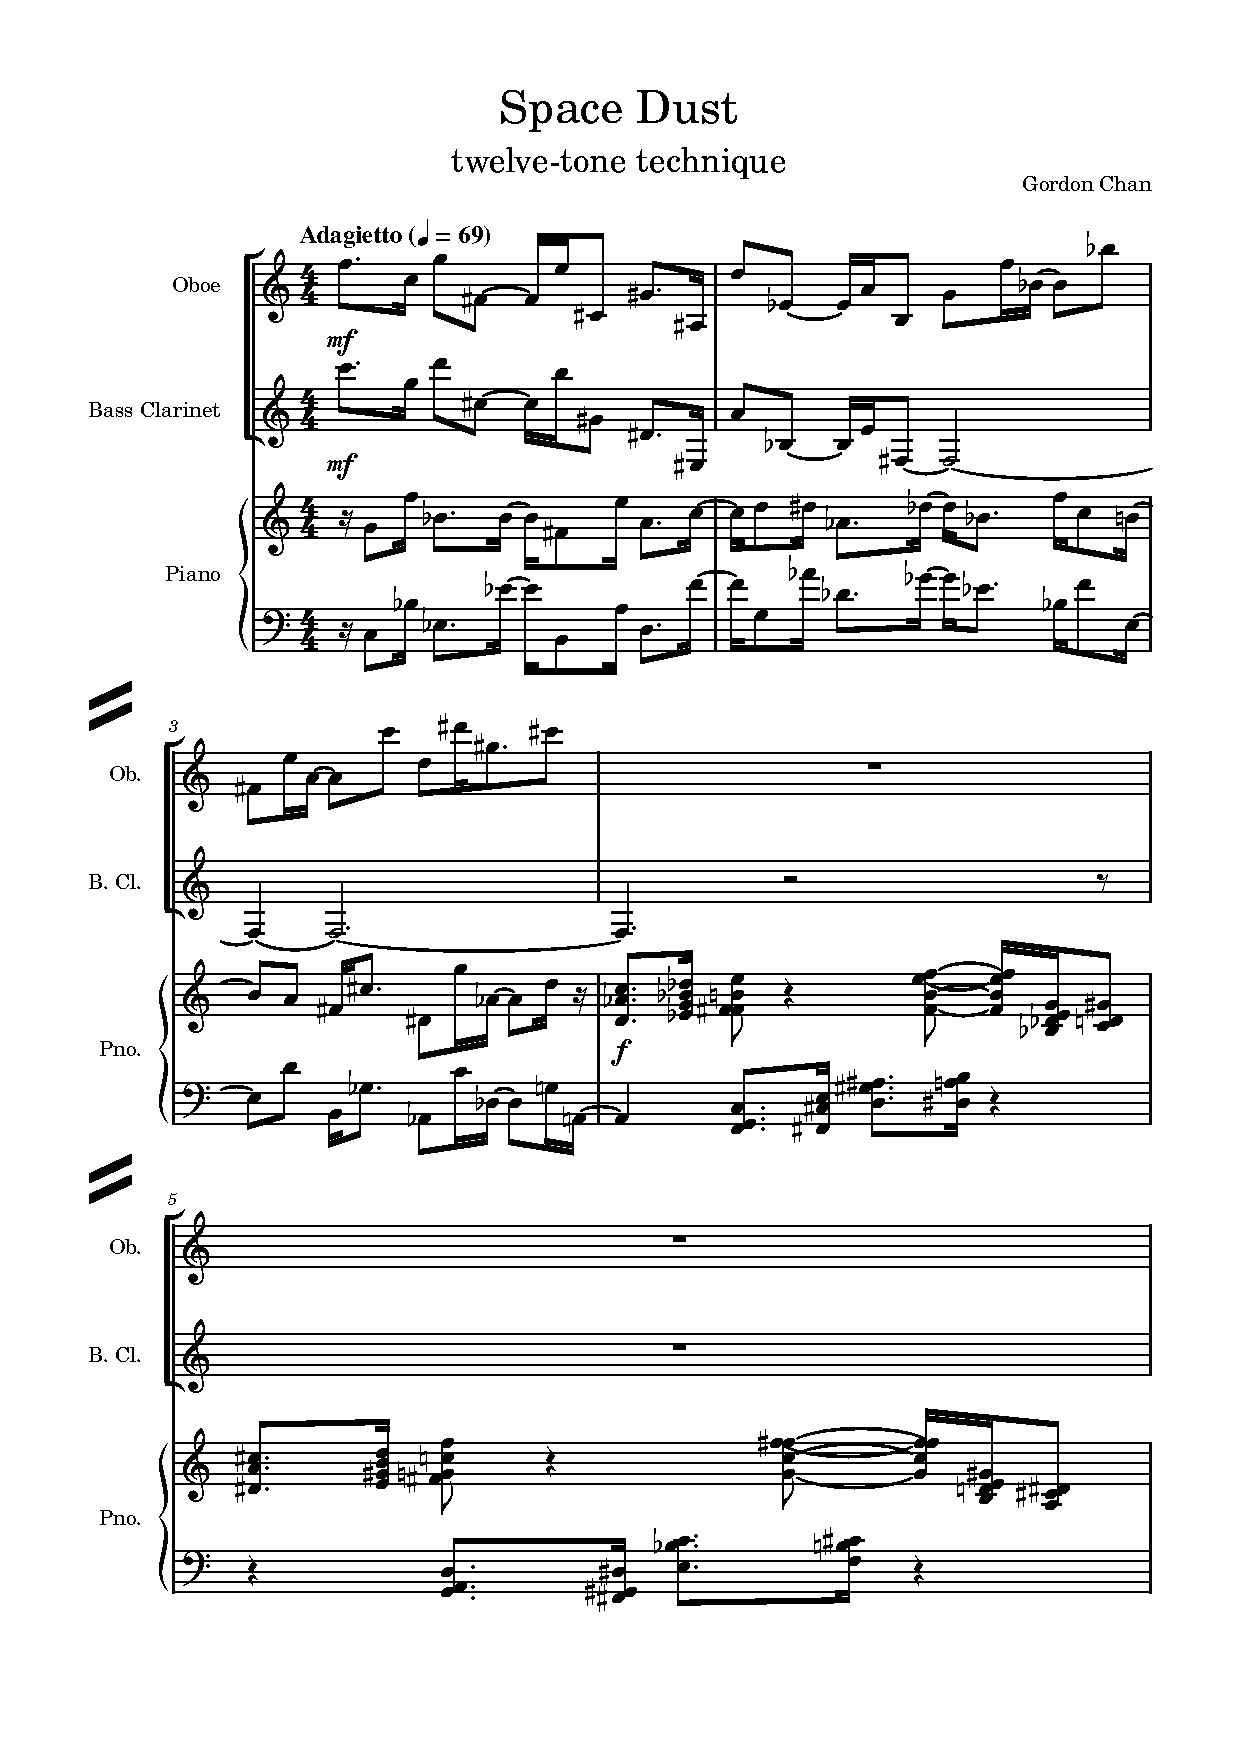
\includepdf[scale=0.9,page=-,pagecommand={\thispagestyle{plain}}]{space_dust.pdf}
\newpage
\begin{center}
\topskip0pt
\vspace*{\fill}
\LARGE
\subsection{Draft 1}
\vspace*{\fill}
%
\end{center}
\newpage
\begin{center}
\topskip0pt
\vspace*{\fill}
\LARGE
\subsection{Draft 2}
\vspace*{\fill}
%
\end{center}
\newpage
\begin{center}
\topskip0pt
\vspace*{\fill}
\LARGE
\subsection{Draft 3}
\vspace*{\fill}
%
\end{center}
\newpage



\newpage
\begin{center}
\topskip0pt
\vspace*{\fill}
\LARGE
    \section{Infree (tone clusters)}
\vspace*{\fill}
%
\end{center}

\newpage

\subsection{Working Timeline}
\begin{center}
	\def\arraystretch{1.5}
\begin{tabular}{|c|l|l|}
	\hline
	Draft&Date&Area explored / Changes made\\
	\hline
	1&27\(^{\text{th}}\) January, 2021
    &Planned characteristic rhythmic motifs and musical progression.\\
	\hline
	2&21\(^{\text{st}}\) March, 2021
    &Enhanced the foreground/background contrast.\\
    &&Worked on the musical direction and building of momentum.\\
    &&Eliminated the doubling of parts.\\
	\hline
	3&2\(^{\text{nd}}\) May, 2021
    &Rewrote instrumental parts, considering practicality,\\
    &&harmonic counterpoints and texture.\\
    &&Reworked notations for ease for reading.\\
	\hline
	Final&1\(^{\text{st}}\) September, 2021
    &Reworked on the usage of clusters, with `tonality'.\\
    &&Varied the musical materials, avoiding exact continuous sequences.\\
    &&Reworked on the pedal markings such that they make sense.\\
	\hline
\end{tabular}
\end{center}

\subsection{Write-up on {\bf Infree}}

\subsubsection{Introduction}

The title of \textbf{Infree} describes the state of not being able to be free.
In this case, it describes the notes and voices in the piece being somewhat
`entangled' with another. It also refers to the effect of tone clusters being
concentrated chunks rather than dispersed. Certain dynamic changes and rhythmic
figures are used to support the character of the work.\\

\subsubsection{Harmony}

In the introductory motif, a E minor tonality is suggested by the flute and
violin.  That somewhat stable tonality then gave way at bar 2 when
the tone clusters are introduced.

There are to main types of tone clusters, the major type and minor type.  The
major type is where the interval between the notes are all major seconds, while
minor type made up of minor seconds. Their are also cluster that do not belong
to any types but counted as bitonal. The following bar are tone clusters made
up of major seconds, followed by a handover of melody to the piano at bar 3,
where the piano play increasingly dissonant chords that are eventually made up
of minor seconds.\\

The piano plays this dissonant passage in triplets from bar 3 to bar 5 until it
descends to the massive clusters at the beginning of bar 6.  At bar 6, the
motif is accompanied by the piano playing powerful bass clusters, which have
more of a percussive effect than harmonic colour.\\

From bar 13 to 16, the piano plays whole-tone clusters. There are four chords,
and they are transpositions of on another.

\subsubsection{Motifs}

At bar 6, the woodwinds and strings play a modified version of the opening
motif, changed in a way that the motif is made of clusters built in major
seconds.  At bars 10 to 12, the piano plays a descending motif, where all the
chords are made of two notes that are a major seventh apart.  While the rest
plays a three bar motif that is constructed by a minim, followed by a quaver
that is displaced a quavers backwards each bar.  The dynamics in these three bars
resembles waves--whenever the piano plays forte, the rest plays softly and vice
versa.\\

In the following four bars, the piano supports the triplet motif in the other
instruments.  That motif is made up of chord of minor seconds which oscillates
up and down for three sets of triplets and then goes downwards for the first
two bars, just descending triplets at the third bar, and descending triplets
that are grouped in twos at the forth.\\

\newpage
\begin{center}
\topskip0pt
\vspace*{\fill}
\LARGE
\subsection{Final Version}
\vspace*{\fill}
%
\end{center}
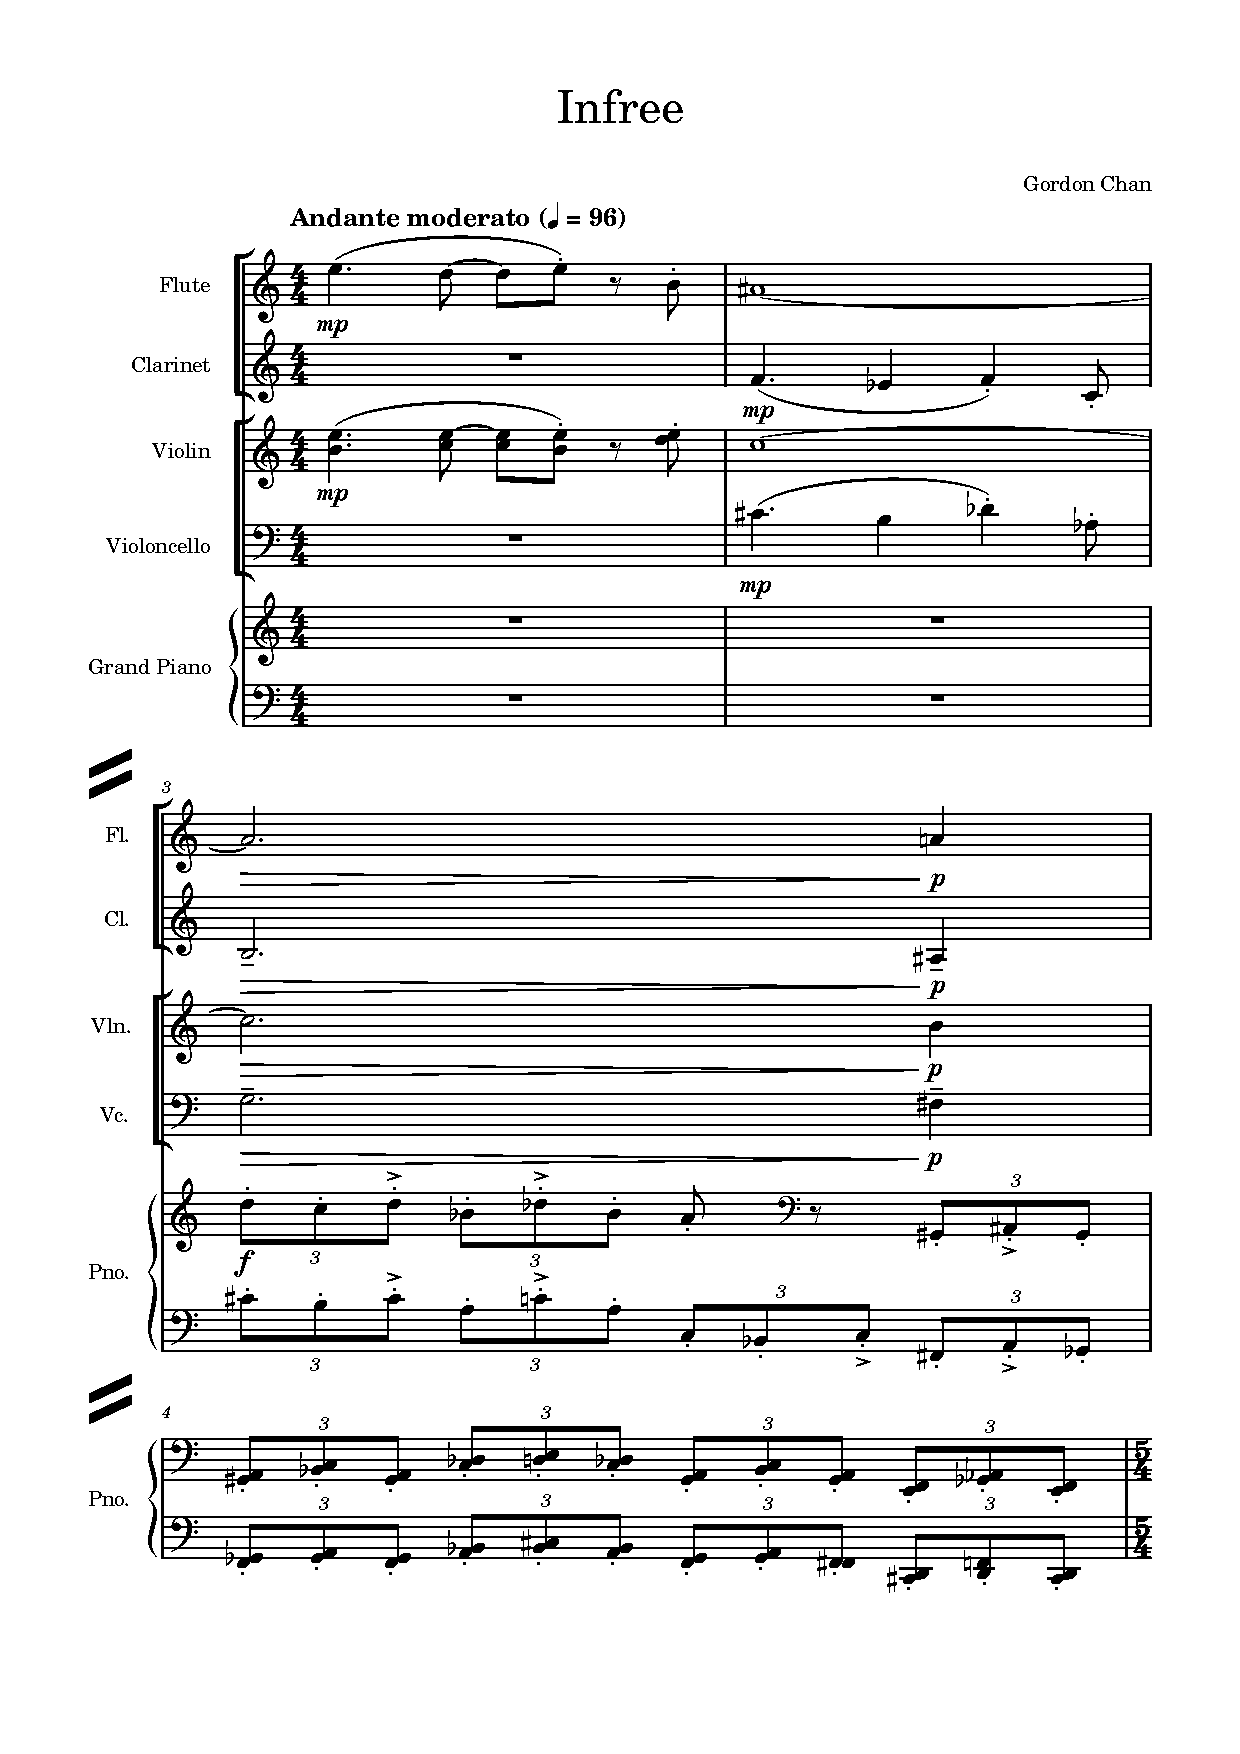
\includepdf[scale=0.9,page=-,pagecommand={\thispagestyle{plain}}]{infree.pdf}
\newpage
\begin{center}
\topskip0pt
\vspace*{\fill}
\LARGE
\subsection{Draft 1}
\vspace*{\fill}
%
\end{center}
\newpage
\emptypage
\emptypage
\emptypage
\emptypage
\emptypage
\emptypage
\emptypage
\emptypage
\emptypage
\emptypage
\emptypage
\emptypage

\begin{center}
\topskip0pt
\vspace*{\fill}
\LARGE
    \section{Wonky Steps (rhythmic counterpoint)}
\vspace*{\fill}
%
\end{center}

\newpage

\subsection{Working Timeline}
\begin{center}
	\def\arraystretch{1.5}
\begin{tabular}{|c|l|l|}
	\hline
	Draft&Date&Area explored / Changes made\\
	\hline
	1&26\(^{\text{th}}\) February, 2021&
    Explored with descending fifth motive, metric displacement, canon.\\
	\hline
    2&2\(^{\text{nd}}\) May, 2021&Greater extent of rhythmic counterpoint.\\
    &&Explored with sense of shifting of space and time.\\
    &&Improved musical direction, notions,\\
    &&imitations between clarinet and piano.\\
	\hline
	3&14\(^{\text{th}}\) July, 2021&Worked on harmonic progressions, sense of tempo increase.\\
	\hline
	Final&31\(^{\text{st}}\) Ang, 2021
    &Worked on sense of suspense before resolution.\\
    &&Improved harmonic direction and harmonic support.\\
    &&Improved counterpoint, sense of arrival, notations.\\
	\hline
\end{tabular}
\end{center}

\subsection{Write-up on {\bf Wonky Steps}}

\subsubsection{Compositional Approach}
The piece, {\bf Wonky Steps}, explores the use of rhythmic counterpoint to
create a sense of instability in the music, in addition to metric displacements
and poly-rhythms.\\

\subsubsection{Structure and Motive Development}
Overall, the work is structured in four sections as such:\\

\begin{center}
	\def\arraystretch{1.5}
\begin{tabular}{|c|c|c|}
	\hline
	Section&Bars&Main Musical Features\\
	\hline
	A&1-11&falling fifth motive and cyclic bass line\\
	\hline
	B&12-16&counterpoint between bass and piano; running notes in clarinet\\
	\hline
	C&17-26&piano rhythm with increasing intensity; reprise of opening motive\\
	\hline
	A\(^\prime\)&27-35&canon in all parts; derived from the retrograded opening motive\\
	\hline
\end{tabular}
\end{center}

The piece opens with a series of falling fifths in both the piano and the
double bass. After that, the double bass plays a bass line based on the melody
in the clarinet part. This rhythm of the clarinet melody is constantly imitated
by the piano throughout bars 5 to 10. A bar of transition is used to change the
rhythmic character at bar 12, to link to a new section. The upper melody in bar
12 played by the clarinet is first played by the piano at bar 11 to foreshadow
the new rhythmic motif.\\

The main theme in section B is taken by the double bass, in a poly-rhythmic
fashion, against the piano part. This theme is based on the same rhythmic idea
introduced a bar before. This theme is set against a new seven-beat rhythm that
emphasises all the even quavers of a bar while right hand plays three quavers
in unison with the double bass at the end of each bar. The three quavers at the
end emphasises the interaction between the piano and double bass parts. The
clarinet then plays a rising Hijaz scale from G4 all the way up to E6, at bar
15.\\

The third section spans from bars 17 to 26. In this section, the double bass
repeats yet another rhythm while outlining the chordal qualities of the bars.
The main effect created in this section however comes from the piano part. The
piano plays an ever increasingly intense rhythm as the music progresses. In
particular, in the first bar of the section, the rhythm consists of two
crochets and two dotted quavers. In the second bar, it changes to three
triplets and two dotted quavers. This pattern continues until on the fourth
bar, there are five quintuplets and two dotted quavers. The frequency of note
heard increases, building up to the climax. As a result, a sense of increasing
excitement is created as the space between each note decreases as the music
progresses. In the subsequent part, the three instruments are playing in unison
to an irregular rhythmic pattern to resolve to an F\(\sharp\) major chord.
Every note other than the last three notes in this section are accented so that
the rhythmic qualities of this motive can be projected clearly. The rhythm used
here consists of two groups of four quadruplets and two groups of four regular
quavers. It is also worthy to note that these groups are arranged with
non-retrogradable rhythm.\\

The forth and final section starts from bar 25 until the end of the work.
Canon is used in this section. It consists of a series of rising fifth motif
with the rhythm derived from retrograding the opening motif. The canon resolves
to a quasi-major chord.\\

\subsubsection{Rhythmic Technique Explored} Rhythmic counterpoint is explored
throughout the work. For example, from bar 3 to bar 11 as the double bass plays
a two-bar rhythmic cycle, with rhythmic interactions between the bass
line and the upper voices. A similar approach is used from bar 13 to 20, where
the bass plays repeated poly-rhythmic motives while piano and clarinet playing
other higher voices.\\

Other techniques are also explored, such as a metric displacement in the
piano's motif from bar 5 to bar 8 where semiquavers rests are constantly being
added each time as the motif repeated, and a non-retrogradable rhythm from bar
21 to 22.\\

\newpage
\begin{center}
\topskip0pt
\vspace*{\fill}
\LARGE
\subsection{Final Version}
\vspace*{\fill}
%
\end{center}
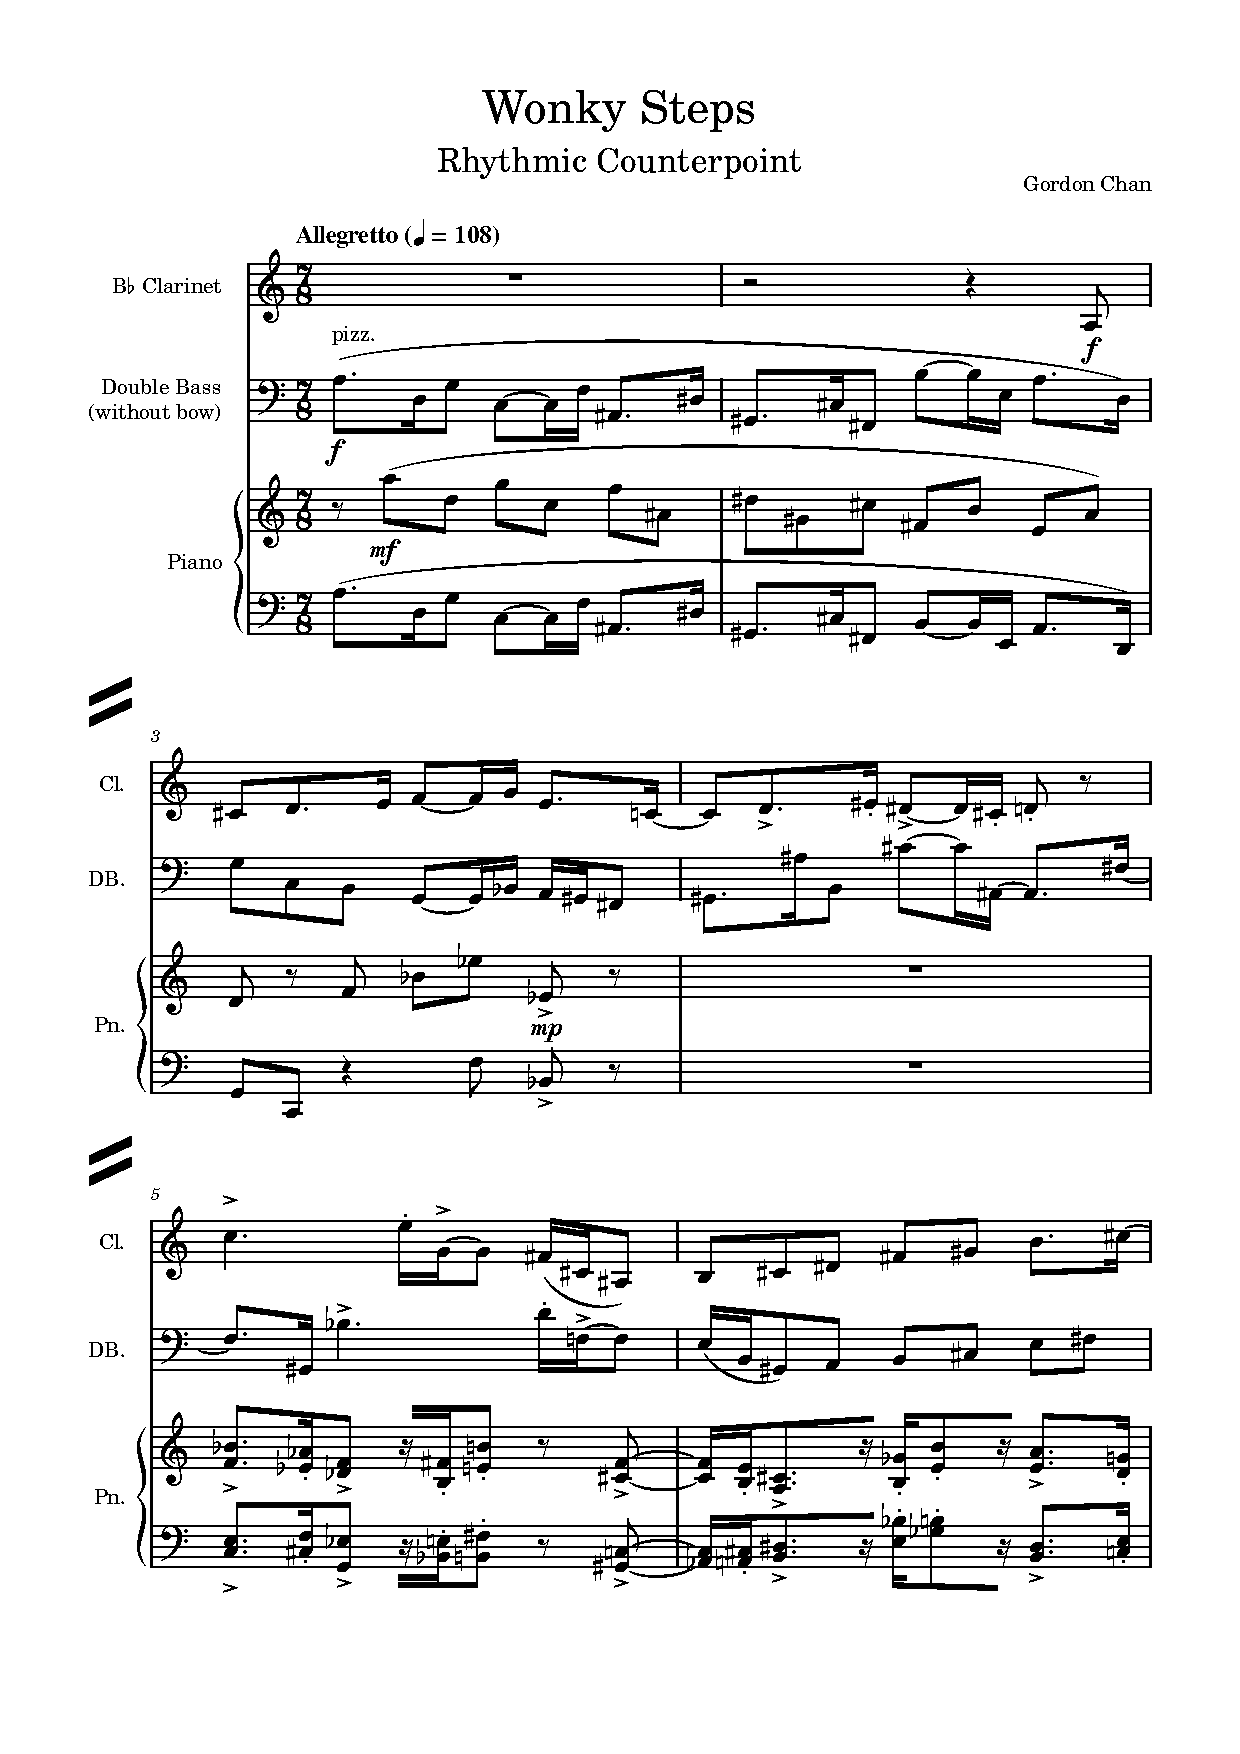
\includepdf[scale=.9,page=-,pagecommand={\thispagestyle{plain}}]{wonky_steps.pdf}
\newpage
\begin{center}
\topskip0pt
\vspace*{\fill}
\LARGE
\subsection{Draft 1}
\vspace*{\fill}
%
\end{center}
\newpage
\emptypage
\emptypage
\emptypage
\emptypage
\emptypage
\begin{center}
\topskip0pt
\vspace*{\fill}
\LARGE
\subsection{Draft 2}
\vspace*{\fill}
%
\end{center}
\newpage
\emptypage
\emptypage
\emptypage
\emptypage
\emptypage
\begin{center}
\topskip0pt
\vspace*{\fill}
\LARGE
\subsection{Draft 3}
\vspace*{\fill}
%
\end{center}

\newpage
\emptypage
\emptypage
\emptypage
\emptypage
\emptypage
\emptypage

\addcontentsline{toc}{part}{Part 2: Composition}

\begin{center}
\topskip0pt
\vspace*{\fill}
\LARGE
    \section{Axiomatic Approximation (for Clarinet Quintet)}
    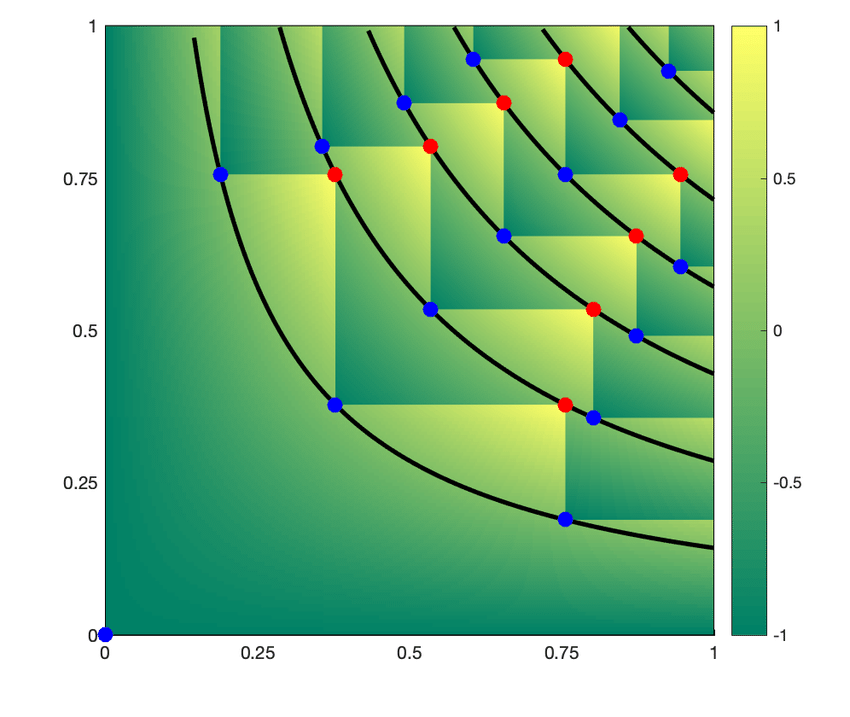
\includegraphics[width=\textwidth]{approximation.png}
\vspace*{\fill}
\end{center}
\subsection{Working Timeline}

\begin{center}
	\def\arraystretch{1.5}
\begin{tabular}{|c|l|l|}
	\hline
	Draft&Date&Area explored / Changes made\\
	\hline
	1&October 2020&
    came up with the three sections\\
	\hline
	2&January 2021&
    improved transition between sections\\
	\hline
	3&March 2021&
    add interruptions in places where it may seem repetitive\\
	\hline
	Final&May 2021&
    fixed notations, overall presentation and improved ending\\
	\hline
\end{tabular}
\end{center}

\subsection{Write-up on {\bf Axiomatic Approximation}}

The title of \textbf{Axiomatic Approximation} comes from the fundamental axioms
in mathematics and the usual idea of approximation in science. There are three
main sections in the work. The first section is a strange waltz in
\(\def\arraystretch{0.0}\begin{array}{c}5\\8\end{array}\). The second section
    is a waltz in \(\def\arraystretch{0.0}\begin{array}{c}6\\8\end{array}\).
        The third section is a swing beat in
\(\def\arraystretch{0.0}\begin{array}{c}4\\4\end{array}\).  The orchestration
    of the work is that of a clarinet quintet, however, unlike the classical
instrumentation where there are two violins and no double bass, I have reduced
one violin in exchange of a double bass, as I feel this there should be a
higher presence of lower register sounds in my work. It is worthy to note that,
the tempos of each section are adjusted in such a way that the pulse is
constant throughout the whole piece. In particular, the pulse is maintained at
69 B.P.M..\\

The first section of the work portray a light-hearted feel. Starting with
cascading pizzicato, the five-beat feel is established at the start of the
section. The pizzicato of the strings may often also be associated with a sense
of cuteness, which sets the mood for the whole section. This section is
referred to as `strange waltz' because five beat is one beat less than the
multiple of three, six. In terms of harmony and key centres, they are rather
unstable to suit the atmosphere. For instance, the piece starts in the key of F
major. However, in bar 11, it is quickly changed to the key of F\(\sharp\)
major. The modulation here utilises the melody as a pivot, as the melody moves
down chromatically from C to B\(\flat\). After that, the same theme is played
in B\(\flat\) with clarinet rhythmic embellishments. The original theme is
played once again by the clarinet and higher strings in a tutti fashion. The
same modulation is repeated from the key of F\(\sharp\) major to the key of G
major. An interruption, however, changes in key abruptly to F major at bar 30
for two bars, and at 32 abruptly to F\(\sharp\) major. This
G\(\to\)F\(\to\)F\(\sharp\) movement is inspired by chromatic enclosure where
the target key is F\(\sharp\) but before reaching the target, the keys a
semitone around the target key is first played. At rehearsal mark C, a chord
progression of
\(\flat\)VII\(\to\)\(\flat\)iii\(\to\)VI\(\to\)ii\(\to\)V\(\to\)I then take the
key from F\(\sharp\) to G. Between the transition of section one and section
two, there is chromatic movements in the strings to modulate from F\(\sharp\)
major to D minor.\\

This second section is a waltz in compound time. It begins with a opening
melody that outlines the overall tonal centre of the whole section. This
opening portion span ten bars, establishing the key of D minor. Then, the cello
and double bass plays in parallel fifths an ostinato pattern that highlights
heavily on the compound meter feel. It also reinforce the harmony. After the
background of the theme has been well introduced into the music, the clarinet
starts play the main melody of this section, accompanied by violin and viola.
The pizzicato played by the upper strings outline the meter and suggest a
harmonic progression which agrees with the melody played by the clarinet. After
the whole melody is played once, the melody is then taken over by the upper
strings, with lower strings playing long bass notes instead of downbeat
quavers. With the melody reiterated once more, the clarinet plays flourishes on
top of the original melody in the form of virtuosic fast scales. These scales
are D Hijaz Kar ascending and D Locrian descending. An interruption soon
follows as the melody is cut off by an abrupt entry of the cello ostinato
pattern. This interruption is responded by the other instruments gradually
until rehearsal mark F where the clarinet, upper strings and lower strings are
each playing phrases that have separate lengths that converge bar 78. The
following two bars, outlining F\(\sharp\), D, B and G in the bass, act as a
cushion to get everyone ready for rehearsal mark G, which leads to the end of
the waltz.\\

The last section is a transition leading into a fast swung passage and frenzy.
The transition is opened by the double bass playing the note G and the clarinet
imitating the melody from the previous section, followed by a characteristic
arpeggio that land on the note G, the same note that the double bass is
playing, just four octaves higher. After that, the violin, viola and cello play
fragments of four quavers that take reference to the first four notes of motif
from the swung section.  The frequency of the appearance of fragments increases
until there is a sudden chromatic, octave displacing four-note motif played by
the clarinet, which is then passed to the other instruments. Then, the five
chord of C is played tutti, signifying the entrance of the swung section. In
the swung, section, there are a few prominent motifs, they are `CABBAGE',
`BEEF' and `EGG'. These motifs are introduced in a quasi-fugue fashion, with
episodes at rehearsal mark I. Also, `EGG's are played as their separate own
episodes. This swung passage leads to the last portion as a frenzy state,
where all of the voices goes into frantic playings, preparing for the end of
the work.

\newpage
\begin{center}
\topskip0pt
\vspace*{\fill}
\LARGE
\subsection{Draft 1}
\vspace*{\fill}
%
\end{center}
\newpage
\begin{center}
\topskip0pt
\vspace*{\fill}
\LARGE
\subsection{Draft 2}
\vspace*{\fill}
%
\end{center}
\newpage
\begin{center}
\topskip0pt
\vspace*{\fill}
\LARGE
\subsection{Draft 3}
\vspace*{\fill}
%
\end{center}
\newpage
\begin{center}
\topskip0pt
\vspace*{\fill}
\LARGE
\subsection{Final Version}
\vspace*{\fill}
%
\end{center}
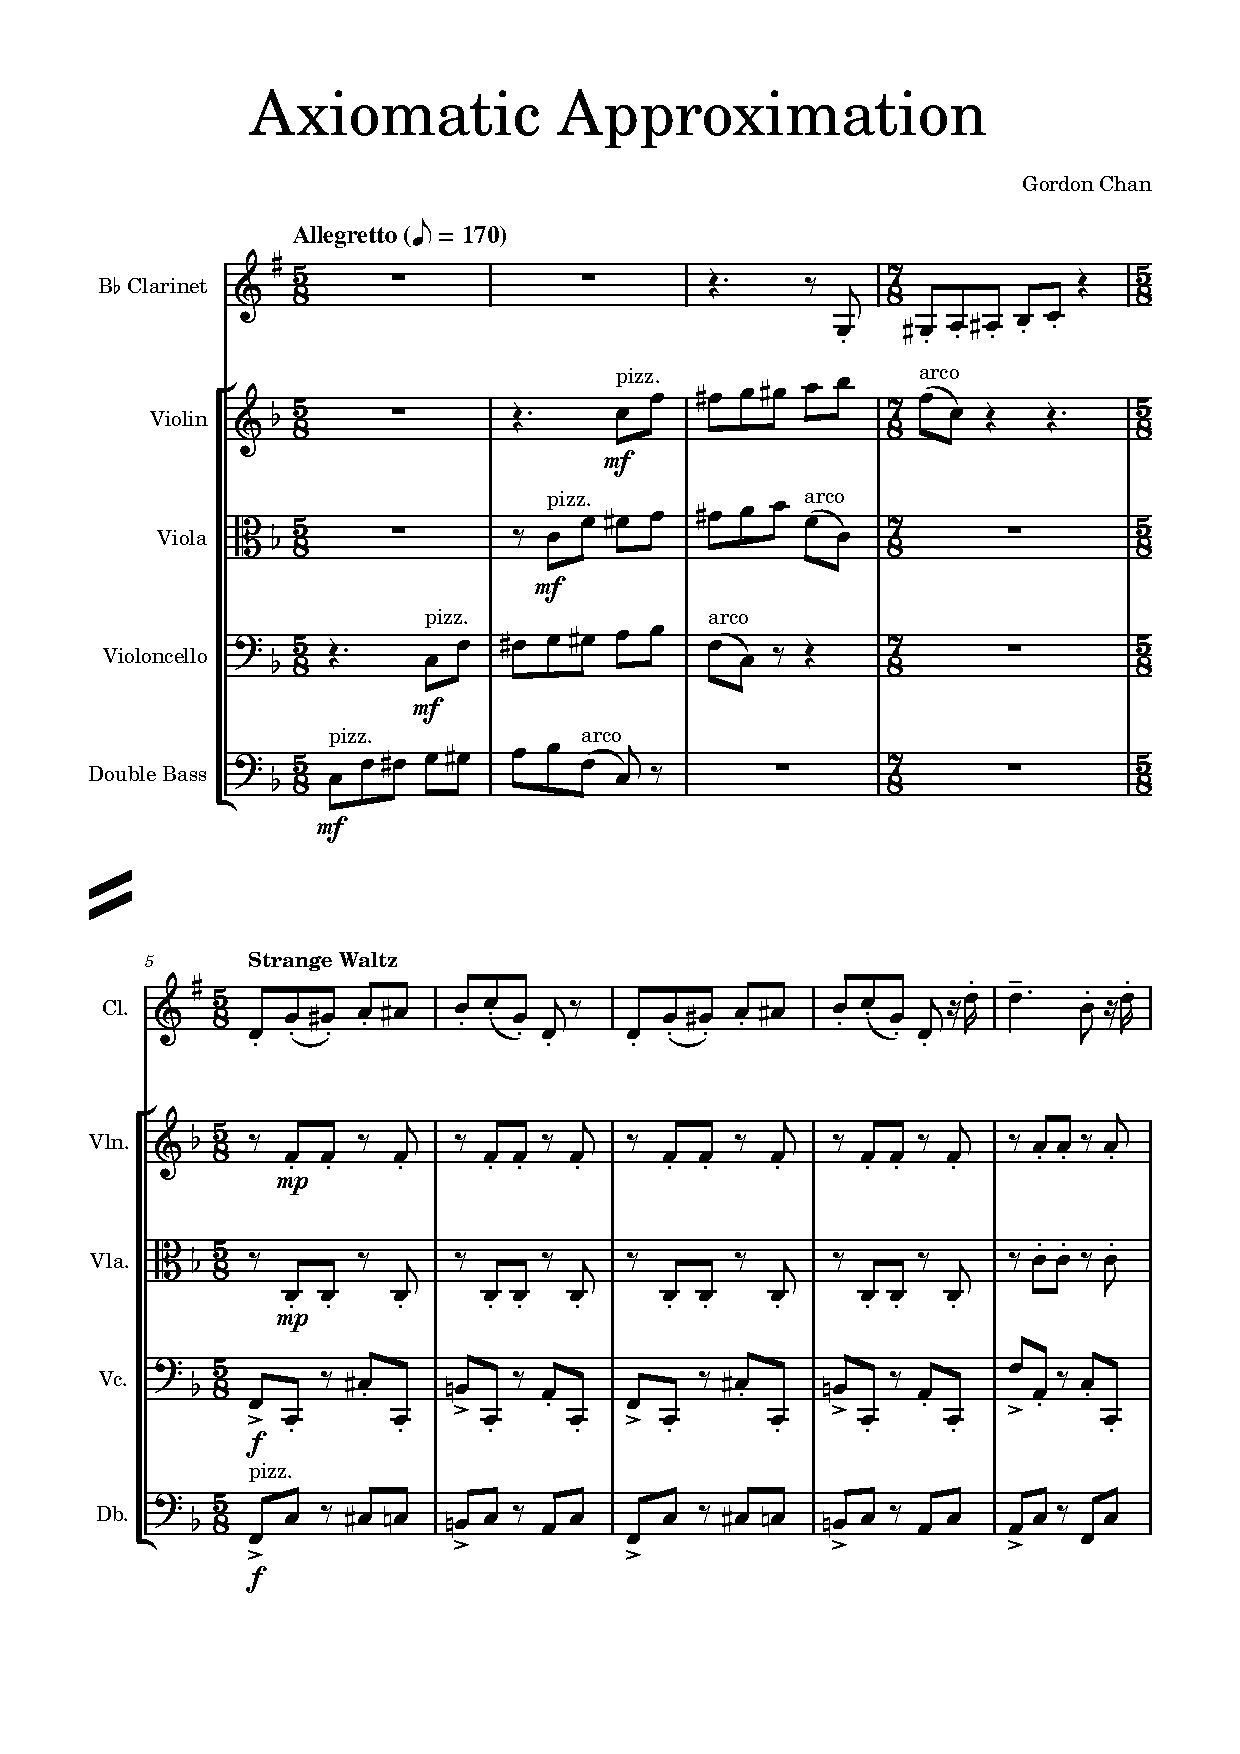
\includepdf[scale=0.9,page=-,pagecommand={\thispagestyle{plain}}]{axiomatic_approximation.pdf}

\section{Acknowledgement}
These are the people whose presence is crucial to the completion of this composition portfolio:
\begin{itemize}
    \item Ms Yick, my composition music teacher, who follow closely on my composition progress and taught me composition techniques;
    \item my uncle, who gives me emotional support;
    \item my aunt, who gives me excellent tips in navigating through junior college life.
\end{itemize}
\section{Epilogue}
Moral integration

\end{document}
